\chapter{Fonksiyonlar}
\label{chap:fonksiyonlar}


\par\smallskip{\sffamily\bfseries\color{cAcc}Öğrenme Hedefleri}\nopagebreak

\begin{itemize}\setlength{\itemsep}{2pt}\setlength{\parskip}{0pt}
\item Fonksiyonu bağıntı olarak tanımlayabilme.
\item Birebir, örten ve eşleme kavramlarını ispatlarla kullanabilme.
\item Bileşke ve ters fonksiyonu kurabilme.
\end{itemize}

\section*{Bölüme Genel Bakış: Fonksiyon Kavramının Serüveni}

Bugün en temel sandığımız fonksiyon kavramı, aslında yüzyıllar süren bir olgunlaşmanın ürünüdür. On yedinci yüzyılda Leibniz ‘fonksiyon’ sözcüğünü bir eğriye bağlı büyüklükler için kullandı; on sekizinci yüzyılda Euler onu bir ‘analitik ifade’ (formül) olarak gördü. Dönüm noktası 1837’de Dirichlet ile geldi: fonksiyon, herhangi bir formüle bağlı olmaksızın ‘her girdiye bir çıktı atayan keyfi bir kural’ olarak tanımlandı. Yirminci yüzyılda Bourbaki bu fikri kümeler diline oturttu: fonksiyon, belirli bir koşulu sağlayan bir bağıntıdır.

Bu tarihsel yolculuk pedagojik olarak öğreticidir: öğrenciler de çoğu zaman fonksiyonu önce ‘formül’ olarak düşünür ve ‘kural’ ya da ‘küme’ görüşüne geçmekte zorlanır. Bu bölüm fonksiyonu bağıntı temelinde tanımlar, birebir/örten/eşleme ayrımını ispatlarla işler ve bileşke, ters, imge gibi işlemleri geliştirir; böylece öğrenci fonksiyonu bir işlem olarak olduğu kadar bir nesne olarak da görebilir hâle gelir.

\section{Tanım}

\begin{tcolorbox}[bookbox,colback=cDef]\textbf{\textsf{\textcolor{cAcc}{Tanım.}}}\quad f: A → B bir fonksiyon, her a ∈ A için tam olarak bir f(a) ∈ B belirleyen bir bağıntıdır. A tanım kümesi, B değer kümesi, f(A) = \{f(a): a ∈ A\} görüntüdür.\end{tcolorbox}

\section{Birebir, Örten, Eşleme}

\begin{tcolorbox}[bookbox,colback=cDef]\textbf{\textsf{\textcolor{cAcc}{Tanım.}}}\quad f birebirdir (injective): f(a₁) = f(a₂) ⇒ a₁ = a₂. f örtendir (surjective): her b ∈ B için f(a) = b olan bir a vardır. Hem birebir hem örten fonksiyon bir eşlemedir (bijection).\end{tcolorbox}

\begin{tcolorbox}[bookbox,colback=cEx]\textbf{\textsf{\textcolor{cAcc}{Örnek.}}}\quad f: ℝ → ℝ, f(x) = 2x + 3 bir eşlemedir.\par\medskip{}Birebir: 2x + 3 = 2y + 3 ⇒ x = y. Örten: verilen y için x = (y − 3)/2 seçilir, f(x) = y. Öyleyse f eşlemedir ve tersi f⁻¹(y) = (y − 3)/2. ∎\end{tcolorbox}

\begin{tcolorbox}[bookbox,colback=cEx]\textbf{\textsf{\textcolor{cAcc}{Örnek.}}}\quad f: ℤ → ℤ, f(n) = 2n birebirdir ama örten değildir (tek sayılar görüntüde yoktur). Bu, tanım ve değer kümesinin fonksiyonun kimliğinin parçası olduğunu gösterir.\end{tcolorbox}

\begin{tcolorbox}[bookbox,colback=cDep]\textbf{\textsf{\textcolor{cAcc}{Muhakeme/Felsefe Derinleştirmesi — Nesne olarak fonksiyon: tarihsel gelişim}}}\quad Fonksiyon kavramı önce ‘bir formül/eğri’ olarak düşünüldü; Dirichlet ile ‘her girdiye bir çıktı atayan keyfi kural’a, Bourbaki ile ‘belirli koşulları sağlayan bir bağıntı (küme)’ tanımına evrildi. Bu, matematiğin bir işlemi (dinamik) bir nesneye (statik küme) dönüştürerek üzerinde muhakeme edebilir kılışının örneğidir — matematikteki ‘varlık’ ve ‘inşa’ sorularının fonksiyonlara uygulanışıdır.\end{tcolorbox}

\begin{figure}[htbp]
\centering
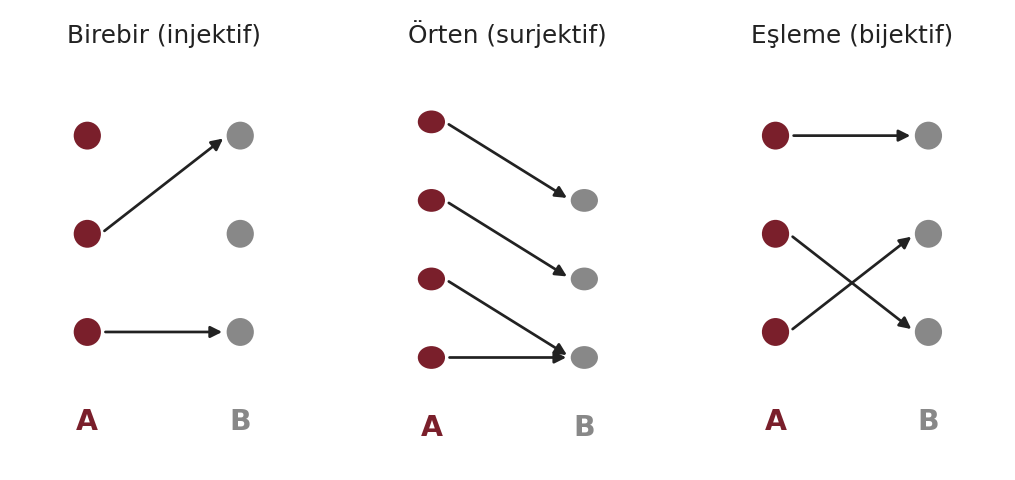
\includegraphics[width=0.91\linewidth]{figs/functions.png}
\caption{Birebir (injektif), örten (surjektif) ve eşleme (bijektif) fonksiyonlar.}
\end{figure}

\section{İleri Örnekler: Bileşke, Ters ve İmge}

Fonksiyon kavramını birkaç somut ispat ve hesapla derinleştirelim. Amaç, birebirlik ve örtenliğin nasıl gösterildiğini ve imge/ön imge kavramlarının nasıl çalıştığını görmektir.

\begin{tcolorbox}[bookbox,colback=cEx]\textbf{\textsf{\textcolor{cAcc}{Örnek.}}}\quad \textbf{Birebirlik ve örtenlik ispatı. }f: ℝ → ℝ, f(x) = x³ bir eşlemedir. Birebir: x³ = y³ ⇒ x = y (küp fonksiyonu kesin artandır). Örten: her y için x = ∛y seçilince f(x) = y. Bu yüzden tersi f⁻¹(y) = ∛y’dir. Buna karşılık f(x) = x² fonksiyonu ℝ → ℝ olarak ne birebirdir (f(−2) = f(2)) ne örtendir (negatif değerler görüntüde yok).\end{tcolorbox}

\begin{tcolorbox}[bookbox,colback=cEx]\textbf{\textsf{\textcolor{cAcc}{Örnek.}}}\quad \textbf{Bileşkenin sırası önemlidir. }f(x) = 2x + 3 ve g(x) = x² için (g ∘ f)(x) = (2x + 3)² iken (f ∘ g)(x) = 2x² + 3. İki bileşke farklıdır; bileşke işlemi genelde değişmeli değildir.\end{tcolorbox}

\begin{tcolorbox}[bookbox,colback=cEx]\textbf{\textsf{\textcolor{cAcc}{Örnek.}}}\quad \textbf{İmge ve ön imge. }f(x) = x² için f(\{−1, 0, 1, 2\}) = \{0, 1, 4\} (imge, tekrarları saymaz). Ön imge f⁻¹(\{4\}) = \{−2, 2\}; f⁻¹(\{−1\}) = ∅, çünkü hiçbir gerçek sayının karesi −1 değildir. Dikkat: burada f⁻¹ ters fonksiyon değil, küme ön imgesidir ve f birebir olmasa da tanımlıdır.\end{tcolorbox}

\begin{tcolorbox}[bookbox,colback=cEx]\textbf{\textsf{\textcolor{cAcc}{Örnek.}}}\quad \textbf{Güvercin yuvası ilkesi. }A ve B sonlu ve |A| > |B| ise A’dan B’ye birebir fonksiyon yoktur: en az iki farklı girdi aynı çıktıya gitmek zorundadır. Örneğin 13 kişiden en az ikisi aynı ayda doğmuştur (13 > 12). Bu basit gözlem, birebirliğin sonlu kümelerde boyutla doğrudan bağını gösterir.\end{tcolorbox}

\begin{tcolorbox}[bookbox,colback=cMis]\textbf{\textsf{\textcolor{cAcc}{Yaygın Kavram Yanılgıları}}}\quad \textbf{“f⁻¹, 1/f demektir.” — }f⁻¹ ters fonksiyondur, çarpımsal ters (1/f) değil. f(x) = 2x + 3 için f⁻¹(x) = (x − 3)/2’dir, 1/(2x + 3) değil.\par\medskip{}\textbf{“Her fonksiyonun tersi vardır.” — }Ters fonksiyon yalnızca eşlemeler (birebir ve örten) için tanımlıdır. Ancak küme ön imgesi f⁻¹(S) her fonksiyon için tanımlıdır.\par\medskip{}\textbf{“İmge ile değer kümesi aynıdır.” — }Görüntü (imge) f(A), değer kümesi B’nin bir alt kümesidir; eşit olması tam da örtenlik demektir.\par\medskip{}\textbf{“Tanım kümesini değiştirmek fonksiyonu değiştirmez.” — }Tanım ve değer kümesi fonksiyonun kimliğinin parçasıdır; x² fonksiyonu ℝ → ℝ ile [0,∞) → [0,∞) olarak farklı fonksiyonlardır (biri eşleme değil, diğeri eşleme).\par\medskip{}\textbf{“f(x + y) = f(x) + f(y) her fonksiyon için geçerlidir.” — }Bu yalnızca doğrusal (toplamsal) fonksiyonlar için doğrudur; f(x) = x² için f(1 + 1) = 4 ≠ f(1) + f(1) = 2.\end{tcolorbox}

\section{Uygulama ve Eğitime Yansıma}

Fonksiyon, hem matematiğin hem de bilgisayar biliminin merkezî kavramıdır: bir program fonksiyonu girdiyi çıktıya götüren bir eşlemedir; veri dönüşümleri, şifreleme (tek yönlü fonksiyonlar) ve makine öğrenmesi modelleri hep fonksiyon dilinde ifade edilir. Öğretimde en verimli köprü, fonksiyonu ‘girdi–çıktı makinesi’ olarak canlandırmak ve grafiğin ‘dikey doğru testi’yle (her girdiye tek çıktı) fonksiyon tanımını görselleştirmektir.

Öğrencilerin en sık zorlandığı nokta, birebirlik ile örtenliği ayırt etmek ve bunların tanım/değer kümesine bağlı olduğunu görmektir. ‘Yatay doğru testi’ (birebirlik) ile ‘dikey doğru testi’ (fonksiyon olma) ayrımını grafik üzerinde çalıştırmak, bu kavramları somutlaştırır ve öğrenciyi biçimsel ispata hazırlar.

\section{Yüksek Lisans Derinleştirmesi: Fonksiyon, Bağıntı ve Sayma}

Biçimsel olarak bir f: A → B fonksiyonu, A × B’nin özel bir alt kümesidir: her a ∈ A için tam olarak bir (a, b) çifti içeren bir bağıntı. Bu tanım, ‘fonksiyon bir kural mıdır yoksa bir nesne midir?’ tartışmasını kesin biçimde çözer — fonksiyon bir kümedir, dolayısıyla üzerinde matematiksel olarak konuşulabilecek bir nesnedir. Böylece Bölüm~\ref{chap:bagintilar}’in bağıntı çatısı, fonksiyonu da içine alır.

Fonksiyonlar aynı zamanda saymanın diliidir. Sonlu A, B için A’dan B’ye tüm fonksiyonların sayısı |B|\textasciicircum{}\{|A|\}’dır; bu yüzden fonksiyon uzayı çoğu zaman Bᴬ ile gösterilir. Özel bir durum, karakteristik fonksiyonlardır: A → \{0, 1\} fonksiyonları ile A’nın alt kümeleri birebir eşlenir (her alt küme, elemanlarına 1, diğerlerine 0 atayan fonksiyona karşılık gelir). Bu eşleme, |P(A)| = 2\textasciicircum{}\{|A|\} eşitliğinin kavramsal açıklamasıdır ve kuvvet kümesinin neden ‘2 üssü’ davrandığını gösterir.

Nihayet, birebir ve örten fonksiyonlar kardinalite karşılaştırmasının aracıdır (Bölüm~\ref{chap:kardinalite}): A’dan B’ye birebir fonksiyon varsa |A| ≤ |B|, bir eşleme varsa |A| = |B| deriz. Güvercin yuvası ilkesi bu dilin sonlu hâlidir; sonsuz kümelerde ise aynı fonksiyon dili, ‘bütün ile parçanın eş güçlü olabilmesi’ gibi sezgiye aykırı ama tutarlı sonuçlara götürür. Böylece fonksiyon kavramı, kümelerden kardinaliteye uzanan teknik omurganın taşıyıcı kirişidir.

\section{Eşlemeler, Permütasyonlar ve Tersler}

Fonksiyonların tersi ve bileşkesi zengin bir yapı kurar. Bir eşlemenin tersi tektir ve f⁻¹ ∘ f = id\_A ile f ∘ f⁻¹ = id\_B eşitliklerini sağlar. Eşleme olmayan fonksiyonlar için ise ‘tek yönlü’ tersler tanımlanabilir: f birebirse bir sol ters (g ∘ f = id\_A), örtense bir sağ ters (f ∘ h = id\_B) vardır. Bu ayrım, birebirlik ile örtenliğin cebirsel karşılığını verir.

\begin{tcolorbox}[bookbox,colback=cEx]\textbf{\textsf{\textcolor{cAcc}{Örnek.}}}\quad \textbf{Permütasyonlar. }Sonlu bir A kümesinin kendisine eşlemeleri, A’nın permütasyonlarıdır; |A| = n ise n! tane vardır. Permütasyonlar bileşke altında bir grup (simetrik grup Sₙ) oluşturur: birim permütasyon vardır, her permütasyonun tersi vardır ve bileşke birleşmelidir. Böylece fonksiyon kavramı doğrudan soyut cebre açılır.\end{tcolorbox}

\begin{tcolorbox}[bookbox,colback=cEx]\textbf{\textsf{\textcolor{cAcc}{Örnek.}}}\quad \textbf{Eşleştirme fonksiyonu. }Cantor’un eşleştirme fonksiyonu π(m, n) = (m + n)(m + n + 1)/2 + n, ℕ × ℕ’den ℕ’ye bir eşlemedir: iki doğal sayıyı tek bir doğal sayıya birebir kodlar. Bu, ‘iki boyutlu’ sayılabilir bilginin ‘tek boyuta’ sığdırılabileceğini gösterir ve Bölüm~\ref{chap:kardinalite}’teki ℕ × ℕ’nin sayılabilirliğinin somut kanıtıdır.\end{tcolorbox}

Kısıtlama (restriction) ve genişletme (extension) de fonksiyonlarla çalışmanın temel araçlarıdır: bir f: A → B fonksiyonu, A’nın bir alt kümesine kısıtlandığında yeni bir fonksiyon verir; tersine, bir fonksiyonu daha geniş bir tanım kümesine tutarlı biçimde genişletmek çoğu zaman matematiğin yaratıcı adımıdır (örneğin faktöriyelin gama fonksiyonuna genişletilmesi). Tüm bu işlemler, fonksiyonu edilgen bir ‘girdi–çıktı kuralı’ olmaktan çıkarıp üzerinde hesap yapılan bir nesneye dönüştürür.

Böylece fonksiyon, dersin teknik omurgasının taşıyıcı kirişidir: kümelerin (Bölüm~\ref{chap:kumeler}) ve bağıntıların (Bölüm~\ref{chap:bagintilar}) üzerine kurulur, kongrüans sınıflarında (Bölüm~\ref{chap:kongruanslar}) iyi tanımlılıkla iş görür ve kardinalite karşılaştırmasının (Bölüm~\ref{chap:kardinalite}) biricik aracıdır. Bu bağlantıları görmek öğrenciye, ayrı ayrı öğrenilen konuların aslında tek bir kavramsal ağın düğümleri olduğunu gösterir — matematiksel olgunluğun en önemli göstergelerinden biri de bu bütünlüğü görebilmektir.

\section{İmge ve Ön Görüntü Cebiri}

Fonksiyonlar yalnızca tek elemanları değil, tüm alt kümeleri de taşır: f, A’nın alt kümelerini B’nin alt kümelerine götürür (imge) ve tersine, B’nin alt kümelerinin ön görüntüsünü A’da belirler. Bu ‘küme düzeyindeki’ davranış, küme işlemleriyle (∪, ∩) ne kadar uyumlu olduğuna göre incelikli bir cebir kurar.

İmge, birleşimle tam uyumludur ama kesişimle yalnızca tek yönlü: f(A ∪ B) = f(A) ∪ f(B) her zaman doğrudur, oysa f(A ∩ B) ⊆ f(A) ∩ f(B) olur ve eşitlik genelde sağlanmaz. Bu asimetri, fonksiyonun ‘birleştirmeyi koruduğunu ama ayırt etmeyi kaybedebileceğini’ söyler.

\begin{tcolorbox}[bookbox,colback=cEx]\textbf{\textsf{\textcolor{cAcc}{Örnek.}}}\quad \textbf{Kesişimde eşitliğin bozulması. }f(x) = x², A = \{1\}, B = \{−1\} alalım. A ∩ B = ∅ olduğundan f(A ∩ B) = ∅. Ama f(A) = \{1\} ve f(B) = \{1\}, dolayısıyla f(A) ∩ f(B) = \{1\}. Görüldüğü gibi ∅ ⊊ \{1\}: eşitlik yok. Sebep açıktır — f birebir olmadığından farklı girdiler (1 ve −1) aynı çıktıya (1) gider ve kesişim ‘yapay olarak’ dolar. f birebir olsaydı eşitlik sağlanırdı.\end{tcolorbox}

Ön görüntü ise çok daha ‘uslu’dur: hem birleşimi hem kesişimi hem de tümleyeni korur. Yani f⁻¹(S ∪ T) = f⁻¹(S) ∪ f⁻¹(T), f⁻¹(S ∩ T) = f⁻¹(S) ∩ f⁻¹(T) ve f⁻¹(Sᶜ) = (f⁻¹(S))ᶜ. Bu düzenli davranış, ön görüntünün neden topoloji ve ölçü kuramında temel araç olduğunu açıklar: süreklilik ‘açık kümelerin ön görüntüsünün açık olması’, ölçülebilirlik ‘ölçülebilir kümelerin ön görüntüsünün ölçülebilir olması’ ile tanımlanır.

\begin{tcolorbox}[bookbox,colback=cEx]\textbf{\textsf{\textcolor{cAcc}{Örnek.}}}\quad \textbf{Ön görüntü kesişimi korur. }x ∈ f⁻¹(S ∩ T) ⇔ f(x) ∈ S ∩ T ⇔ f(x) ∈ S ∧ f(x) ∈ T ⇔ x ∈ f⁻¹(S) ∧ x ∈ f⁻¹(T) ⇔ x ∈ f⁻¹(S) ∩ f⁻¹(T). Her adım bir mantıksal eşdeğerlik olduğundan eşitlik kesindir; ön görüntünün üstünlüğü, tam da bu ‘⇔’ zincirinin hiç kırılmamasıdır. ∎\end{tcolorbox}

Gösterge (karakteristik) fonksiyonları bu resmi tamamlar. Bir A ⊆ U alt kümesinin gösterge fonksiyonu χ\_A, A’nın elemanlarına 1, diğerlerine 0 atar. Küme işlemleri bu fonksiyonların aritmetiğine çevrilir: χ\_\{A∩B\} = χ\_A · χ\_B ve χ\_\{A∪B\} = χ\_A + χ\_B − χ\_A · χ\_B. Böylece küme cebri, bir fonksiyon aritmetiğine dönüşür; bu, olasılık kuramında (bir olayın gösterge fonksiyonunun beklenen değeri, olasılığıdır) ve kombinatorikte sürekli kullanılan güçlü bir tekniktir.

Bu bölüm, fonksiyonun neden yalnızca ‘girdi–çıktı’ değil, aynı zamanda kümeler arası bir taşıyıcı olduğunu gösterir. İmge ve ön görüntünün farklı davranışları, birebirlik ve örtenlik kavramlarını yeni bir açıdan aydınlatır ve Bölüm~\ref{chap:kumeler}’un küme cebri ile Bölüm~\ref{chap:kardinalite}’ün kardinalite argümanlarını fonksiyon diliyle birbirine bağlar. Öğretmen adayı için buradaki incelik, ‘fonksiyon uygularken neyin korunup neyin kaybolduğunu’ bilmenin, ileri matematikteki pek çok tanımın (süreklilik, ölçülebilirlik) doğal olarak anlaşılmasını sağlamasıdır.

\begin{tcolorbox}[bookbox,colback=cDef]\textbf{\textsf{\textcolor{cAcc}{Tarihsel Not}}}\quad Fonksiyon kavramının modern tanımı, 1837’de Peter Gustav Lejeune Dirichlet ile netleşti: bir fonksiyon, herhangi bir formüle bağlı olmaksızın ‘her girdiye tam bir çıktı atayan’ kuraldır. Dirichlet, bunu göstermek için ünlü örneğini verdi — rasyonel sayılarda 1, irrasyonellerde 0 değerini alan, hiçbir formülle yazılamayan ama tümüyle geçerli bir fonksiyon. Bu ‘keyfi kural’ görüşü, fonksiyonu bir eğri ya da cebirsel ifadeyle özdeşleştiren eski anlayışı geride bıraktı ve modern analize giden yolu açtı.\end{tcolorbox}

\section{Fonksiyonları Görmek: Ok Diyagramları, Grafikler ve Tersler}

Bir fonksiyon üç farklı biçimde temsil edilebilir: bir kural (formül), bir ok diyagramı (sonlu kümelerde) ve bir grafik (reel fonksiyonlarda). Birebirlik, örtenlik, bileşke ve ters kavramlarının her biri bu temsillerin birinde çok daha kolay görülür. İyi bir öğretim, öğrencinin temsiller arasında rahatça geçiş yapabilmesini hedefler.

\begin{figure}[htbp]
\centering
\begin{tikzpicture}[e/.style={circle,fill=bar,inner sep=1.3pt},>={Stealth[length=5pt]}]
\foreach \x/\n/\lab/\k/\col in {0/A/{a_1,a_2,a_3}/3/acc,2.6/B/{b_1,b_2,b_3,b_4}/4/warm,5.2/C/{c_1,c_2,c_3}/3/grn}{
  \draw[\col,line width=.9pt,fill=\col!8] (\x,0) ellipse (.6 and 1.45);
  \node[font=\sffamily\bfseries\small,text=\col] at (\x,1.75) {$\n$};
  \foreach \t [count=\i] in \lab {\pgfmathsetmacro{\yy}{((\k+1)/2-\i)*0.72}\node[e] (\n\i) at (\x,\yy) {}; \node[font=\scriptsize,anchor=east] at (\x-.08,\yy) {$\t$};}
}
\foreach \a/\b in {1/1,2/3,3/4}{\draw[->,acc,line width=.8pt] (A\a)--(B\b);}
\foreach \a/\b in {1/1,2/1,3/2,4/3}{\draw[->,warm,line width=.8pt] (B\a)--(C\b);}
\node[font=\sffamily\small,text=acc] at (1.3,-1.85) {$f$ (birebir, örten değil)};
\node[font=\sffamily\small,text=warm] at (3.9,-1.85) {$g$ (örten, birebir değil)};
\draw[->,bar,line width=.9pt] (0,-2.35) to[bend right=14] node[below,font=\sffamily\small]{$g\circ f$: $a_1\mapsto c_1,\ a_2\mapsto c_2,\ a_3\mapsto c_3$ (bir eşleme!)} (5.2,-2.35);
\end{tikzpicture}
\caption{Ok diyagramlarıyla bileşke. $f$ birebir ama $b_2$’ye ok gelmediğinden örten değildir; $g$ örtendir ama $b_1$ ve $b_2$’yi aynı yere götürür. Buna rağmen $g\circ f$ bir eşlemedir: bileşenlerin kusurları birbirini ‘götürebilir’. $g\circ f$’nin birebir olması $f$’nin, örten olması ise $g$’nin karşılık gelen özelliğini zorunlu kılar (Alıştırma 4).}
\end{figure}

\begin{figure}[htbp]
\centering
\begin{tikzpicture}
\begin{axis}[width=.62\linewidth,height=.62\linewidth,xmin=-2.2,xmax=4.2,ymin=-2.2,ymax=4.2,axis lines=middle,
  xlabel={$x$},ylabel={$y$},tick label style={font=\sffamily\scriptsize},samples=120,
  legend style={at={(0.03,0.97)},anchor=north west,font=\sffamily\scriptsize,fill=white,draw=none}]
\addplot[acc,line width=1.2pt,domain=-2.2:1.43]{exp(x)}; \addlegendentry{$y=e^x$}
\addplot[warm,line width=1.2pt,domain=0.11:4.2]{ln(x)}; \addlegendentry{$y=\ln x$}
\addplot[mid,dashed,domain=-2.2:4.2]{x}; \addlegendentry{$y=x$}
\addplot[only marks,mark=*,mark size=1.6pt,acc] coordinates {(1,2.718)};
\addplot[only marks,mark=*,mark size=1.6pt,warm] coordinates {(2.718,1)};
\draw[dotted,bar] (axis cs:1,2.718)--(axis cs:2.718,1);
\end{axis}
\end{tikzpicture}
\caption{Bir eşleme ile tersinin grafikleri $y=x$ doğrusuna göre birbirinin yansımasıdır: $(1,e)$ noktası $(e,1)$ noktasına gider. Yatay her doğru $e^x$ grafiğini en fazla bir kez kestiği için $e^x$ birebirdir; ama $y\le0$ doğrularını hiç kesmediğinden $\mathbb R\to\mathbb R$ olarak örten değildir. Ters, ancak değer kümesi $(0,\infty)$ alındığında tanımlıdır.}
\end{figure}

\begin{ornek}[\textbf{Fonksiyonları saymak.}]
$|A|=3$, $|B|=4$ olsun. $A$’nın her elemanı için 4 seçenek olduğundan $4^3=64$ fonksiyon vardır. Birebir olanlarda seçenekler her adımda bir azalır: $4\cdot3\cdot2=24$. Örten fonksiyon yoktur, çünkü üç elemanlı bir küme dört elemanın hepsine ulaşamaz. Ters yönde $|A|=4$, $|B|=3$ için $3^4=81$ fonksiyonun kaçının örten olduğunu içerme–dışlama (Bölüm~\ref{chap:kumeler}) verir: bir elemanı ıskalayan fonksiyonlar $3\cdot2^4$, iki elemanı ıskalayanlar $3\cdot1^4$ olduğundan örten fonksiyon sayısı $81-48+3=36$’dır. Sayma sonuçları, sonlu kümelerde ‘birebir $\Rightarrow |A|\le|B|$’ ve ‘örten $\Rightarrow |A|\ge|B|$’ ilkelerinin nicel yüzüdür; bu ilkeler Bölüm~\ref{chap:kardinalite}’te sonsuz kümelerin karşılaştırılmasının tanımı olacaktır.
\end{ornek}

\begin{yanilgi}[Yaygın Kavram Yanılgıları]
\textbf{‘$f^{-1}(x)=\dfrac1{f(x)}$’dir.’} — Ters fonksiyon ile çarpımsal ters farklıdır. $f(x)=2x$ için $f^{-1}(x)=x/2$, ama $1/f(x)=1/(2x)$’tir. Gösterimdeki $-1$ üssü iki farklı işlem için kullanılır.

\smallskip
\textbf{‘$f^{-1}(D)$ yazabilmek için $f$ tersinir olmalıdır.’} — Ön görüntü $f^{-1}(D)=\{x: f(x)\in D\}$ her fonksiyon için tanımlıdır. $f(x)=x^2$ için $f^{-1}(\{4\})=\{-2,2\}$ ve $f^{-1}(\{-1\})=\varnothing$’dir; oysa ters fonksiyon yoktur.

\smallskip
\textbf{‘Her formül bir fonksiyon tanımlar.’} — $y^2=x$ bağıntısı her $x>0$’a iki $y$ karşılık getirdiğinden ($x$’ten $y$’ye) bir fonksiyon değildir; ‘dikey doğru testi’ bu kusuru grafikte gösterir. Tanım kümesi ve değer kümesi belirtilmeden ‘fonksiyon’ sözü eksiktir.

\smallskip
\textbf{‘$(g\circ f)^{-1}=g^{-1}\circ f^{-1}$’dir.’} — Sıra ters çevrilir: $(g\circ f)^{-1}=f^{-1}\circ g^{-1}$. Önce giyilen çorap, en son çıkarılır.
\end{yanilgi}

\begin{sinif}[Sınıfta · Üç temsil, bir fonksiyon]
Gruplara aynı fonksiyonun üç temsilinden yalnızca birini verin (formül, ok diyagramı ya da grafik) ve diğer ikisini kurmalarını isteyin. Ardından her grup, ‘Birebir mi? Örten mi? Tersi var mı?’ sorularını kendi başlangıç temsilinde yanıtlasın ve hangi temsilde yanıtın en kolay görüldüğünü tartışsın. Tipik bulgu: birebirlik grafikte (yatay doğru testi), örtenlik ok diyagramında (ok gelmeyen eleman), ters ise formülde (denklemi $x$ için çözme) daha kolay görülür.
\end{sinif}

\section*{Alıştırmalar}

\reviewitem{1}{f: ℝ → (−1, 1), f(x) = x / (1 + |x|) fonksiyonunun bir eşleme olduğunu gösterin ve tersini bulun.}

\reviewitem{2}{|A| = |B| = n (sonlu) ise, birebir bir f: A → B fonksiyonunun aynı zamanda örten olduğunu gösterin.}

\reviewitem{3}{Herhangi bir f: A → B ve alt kümeler için f(A₁ ∪ A₂) = f(A₁) ∪ f(A₂) eşitliğini kanıtlayın.}

\reviewitem{4}{g ∘ f bileşkesi birebirse, f’nin de birebir olduğunu gösterin. Aynı koşulda g birebir olmak zorunda mıdır?}

\reviewitem{5}{İki küme için χ\_\{A △ B\} = χ\_A + χ\_B (mod 2) olduğunu gösterin.}

\section*{Bölüm Özeti}

\begin{itemize}\setlength{\itemsep}{2pt}\setlength{\parskip}{0pt}
\item Fonksiyon, her girdiye tek çıktı atayan özel bir bağıntıdır.
\item Birebir/örten/eşleme ayrımı, fonksiyonun tersinin var olup olmadığını belirler.
\item Tanım ve değer kümesi fonksiyonun kimliğinin parçasıdır.
\end{itemize}

\section*{Gözden Geçirme Soruları}

\reviewitem{1}{f(x) = x² fonksiyonunun ℝ → ℝ ve [0, ∞) → [0, ∞) tanımlarında birebir/örtenlik durumunu karşılaştırınız.}

\reviewitem{2}{İki birebir fonksiyonun bileşkesinin de birebir olduğunu ispatlayınız.}

\section*{Çoktan Seçmeli Sorular}

\mcqq{1}{f(a₁) = f(a₂) ⇒ a₁ = a₂ koşulu neyi tanımlar?}

\mcqo{A}{Örten}

\mcqo{B}{Birebir}

\mcqo{C}{Sabit}

\mcqo{D}{Eşleme}

\mcqa{B}{Bu koşul birebirliğin (injektifliğin) tanımıdır.}

\mcqq{2}{Bir fonksiyonun tersinin var olması için gereken nedir?}

\mcqo{A}{Yalnızca birebir}

\mcqo{B}{Yalnızca örten}

\mcqo{C}{Eşleme (birebir ve örten)}

\mcqo{D}{Sürekli olması}

\mcqa{C}{Ters, ancak eşleme (birebir ve örten) fonksiyonda vardır.}

\mcqq{3}{f: ℤ → ℤ, f(n) = 2n için hangisi doğrudur?}

\mcqo{A}{Birebir, örten değil}

\mcqo{B}{Örten, birebir değil}

\mcqo{C}{Eşleme}

\mcqo{D}{Sabit}

\mcqa{A}{2n birebirdir ama tek sayılar görüntüde yok: örten değil.}

\mcqq{4}{Fonksiyon nasıl tanımlanır?}

\mcqo{A}{Her girdiye en az bir çıktı}

\mcqo{B}{Her girdiye tam bir çıktı}

\mcqo{C}{Her çıktıya bir girdi}

\mcqo{D}{Herhangi bir bağıntı}

\mcqa{B}{Fonksiyon her girdiye tam bir çıktı atar.}

\mcqq{5}{Örten (surjective) fonksiyon nedir?}

\mcqo{A}{f(a₁)=f(a₂) ⇒ a₁=a₂}

\mcqo{B}{Her b ∈ B için f(a) = b olan bir a vardır}

\mcqo{C}{Sabit fonksiyon}

\mcqo{D}{İkili bağıntı}

\mcqa{B}{Örtenlik: her hedef değere ulaşan bir girdi vardır.}

\mcqq{6}{f: ℝ → ℝ, f(x) = 2x + 3 nedir?}

\mcqo{A}{Yalnızca birebir}

\mcqo{B}{Yalnızca örten}

\mcqo{C}{Eşleme}

\mcqo{D}{Sabit}

\mcqa{C}{2x+3 hem birebir hem örten: eşleme.}

\mcqq{7}{f: ℝ → ℝ, f(x) = x² nedir?}

\mcqo{A}{Birebir}

\mcqo{B}{Örten}

\mcqo{C}{Eşleme}

\mcqo{D}{Ne birebir ne örten}

\mcqa{D}{x² ℝ’de ne birebir (±) ne örtendir (negatifler yok).}

\mcqq{8}{İki birebir fonksiyonun bileşkesi nasıldır?}

\mcqo{A}{Birebirdir}

\mcqo{B}{Örtendir}

\mcqo{C}{Sabittir}

\mcqo{D}{Tanımsızdır}

\mcqa{A}{Birebir fonksiyonların bileşkesi birebirdir.}

\mcqq{9}{f: A → B fonksiyonunda B neye karşılık gelir?}

\mcqo{A}{Görüntü}

\mcqo{B}{Değer kümesi}

\mcqo{C}{Çekirdek}

\mcqo{D}{Grafik}

\mcqa{B}{B, fonksiyonun değer kümesidir.}

\mcqq{10}{Görüntü kümesi f(A) nedir?}

\mcqo{A}{A}

\mcqo{B}{\{f(a): a ∈ A\}}

\mcqo{C}{B}

\mcqo{D}{∅}

\mcqa{B}{Görüntü, \{f(a): a∈A\} kümesidir.}

\mcqq{11}{f(x) = x², [0, ∞) → [0, ∞) olarak nedir?}

\mcqo{A}{Birebir değil}

\mcqo{B}{Örten değil}

\mcqo{C}{Eşleme}

\mcqo{D}{Sabit}

\mcqa{C}{Tanım/değer kümesi kısıtlanınca x² bir eşleme olur.}

\mcqq{12}{f birebir değilse ne olur?}

\mcqo{A}{Örten olur}

\mcqo{B}{Tersi (fonksiyon olarak) tanımlanamaz}

\mcqo{C}{Sabit olur}

\mcqo{D}{Sürekli olur}

\mcqa{B}{Birebir değilse ters tek değerli olmaz, tanımlanamaz.}

\mcqq{13}{f: \{1,2,3\} → \{a,b\} bir fonksiyon örten olabilir mi?}

\mcqo{A}{Evet ama birebir olamaz}

\mcqo{B}{Hayır}

\mcqo{C}{Yalnızca birebir olabilir}

\mcqo{D}{Hiçbiri}

\mcqa{A}{3 > 2 olduğundan örten olabilir ama birebir olamaz.}

\mcqq{14}{Bileşke (g ∘ f)(x) neye eşittir?}

\mcqo{A}{f(g(x))}

\mcqo{B}{g(f(x))}

\mcqo{C}{f(x)·g(x)}

\mcqo{D}{f(x)+g(x)}

\mcqa{B}{Bileşke önce f sonra g: g(f(x)).}

\mcqq{15}{Fonksiyon bir bağıntı olarak nasıl görülür?}

\mcqo{A}{Her a için birden çok (a, b)}

\mcqo{B}{Her a için tam bir (a, b) içerir}

\mcqo{C}{Bağıntı değildir}

\mcqo{D}{Simetriktir}

\mcqa{B}{Fonksiyon, her a için tek (a,b) içeren bağıntıdır.}

\mcqq{16}{Sabit fonksiyon f(x) = c genelde nasıldır?}

\mcqo{A}{Eşleme}

\mcqo{B}{Birebir}

\mcqo{C}{Genelde ne birebir ne örten}

\mcqo{D}{Örten}

\mcqa{C}{Sabit fonksiyon genelde ne birebir ne örtendir.}

\mcqq{17}{f bir eşleme ise sonlu A ve B için hangisi doğrudur?}

\mcqo{A}{|A| < |B|}

\mcqo{B}{|A| = |B|}

\mcqo{C}{|A| > |B|}

\mcqo{D}{İlişkisiz}

\mcqa{B}{Sonlu kümeler arası eşleme boyutları eşitler.}

\mcqq{18}{Ters fonksiyon f⁻¹ ne yapar?}

\mcqo{A}{A’dan A’ya gider}

\mcqo{B}{B’den A’ya gider; f(a)=b ⇒ f⁻¹(b)=a}

\mcqo{C}{f ile aynıdır}

\mcqo{D}{Sabittir}

\mcqa{B}{f⁻¹, çıktıyı girdisine geri gönderir.}

\mcqq{19}{f: ℤ → ℤ, f(n) = n + 1 nedir?}

\mcqo{A}{Birebir değil}

\mcqo{B}{Örten değil}

\mcqo{C}{Eşleme}

\mcqo{D}{Sabit}

\mcqa{C}{n+1 hem birebir hem örten: eşleme.}

\mcqq{20}{Fonksiyon kavramı tarihsel olarak (Dirichlet) nasıl gelişti?}

\mcqo{A}{Yalnızca formül olarak kaldı}

\mcqo{B}{Keyfi bir atama kuralına genişledi}

\mcqo{C}{Yalnızca eğri olarak}

\mcqo{D}{Hiç değişmedi}

\mcqa{B}{Dirichlet ile fonksiyon ‘keyfi atama kuralı’na genişledi.}


\clearpage

\clearpage